\documentclass[11pt,a4paper,ngerman]{article}
\usepackage[bottom=2.5cm,top=2.5cm]{geometry} 
\usepackage{babel}
\usepackage[utf8]{inputenc} 
\usepackage[T1]{fontenc} 
\usepackage{ae} 
\usepackage{amssymb} 
\usepackage{amsmath}
\usepackage{amsthm} 
\usepackage{graphicx}
\usepackage{fancyhdr}
\usepackage{fancyref}
\usepackage{listings}
\usepackage{xcolor}
\usepackage{tikz}
\usepackage{paralist}

\usepackage[pdftex, bookmarks=false, pdfstartview={FitH}, linkbordercolor=white]{hyperref}
\usepackage{fancyhdr}
\pagestyle{fancy}
\fancyhead[C]{Höhere Algorithmik II}
\fancyhead[L]{Übung 2}
\fancyhead[R]{SoSe 2013}
\fancyfoot{}
\fancyfoot[L]{}
\fancyfoot[C]{\thepage \hspace{1px} of \pageref{LastPage}}
\renewcommand{\footrulewidth}{0.5pt}
\renewcommand{\headrulewidth}{0.5pt}
\setlength{\parindent}{0pt} 
\setlength{\headheight}{0pt}

\date{}
\title{Übung 2}
\author{Max Wisniewski, Alexander Steen}


%%
%% Enviroments for proofs and lemmas
%%
\newtheorem{lemma}{\bfseries Claim}

\begin{document}

\lstset{language=Pascal, basicstyle=\ttfamily\fontsize{10pt}{10pt}\selectfont\upshape, commentstyle=\rmfamily\slshape, keywordstyle=\rmfamily\bfseries, breaklines=true, frame=single, xleftmargin=3mm, xrightmargin=3mm, tabsize=2, mathescape=true}

\renewcommand{\figurename}{Figure}

\maketitle
\thispagestyle{fancy}

%%%%%%%%%%%%%%%%%%%%%%%%%%%%%%%%%%%%%%%%%%%
%%%%% Aufgabe 1 %%%%%%%%%%%%%%%%%%%%%%%%%%%
\subsection*{Aufgabe 1}
Gesucht ist ein $O(M(n))$-Algorithmus zur Bestimmung des Betrags der Determinanten, wobei $M(n)$ die Anzahl
der arithmetischen Operationen für die Matrizenmultiplikation von $n \times n$-Matrizen ist. \\

\textbf{Lösung}: \\
Sei $A$ eine invertierbare $n \times n$-Matrix. Wir zerteilen die Matrix wie in der VL in folgende Teile:

\begin{equation*}
A = XYZ = \left( \begin{array}{cc}
          I & 0 \\
          A_{21}A_{11}^{-1} & I
          \end{array} \right)
          \left( \begin{array}{cc}
          A_{11} & 0 \\
          0 & D
          \end{array} \right)
          \left( \begin{array}{cc}
          I & A_{11}^{-1}A_{12} \\
          0 & I
          \end{array} \right)
\end{equation*}

wobei

\begin{equation*}
A = \left( \begin{array}{cc}
          A_{11} & A_{12} \\
          A_{21} & A_{22}
    \end{array} \right), \quad
D = A_{22} - A_{21}A_{11}^{-1}A_{12}
\end{equation*}
Wir nehmen vorerst an, dass $A_{11}$ ebenfalls invertierbar ist. Wir kommen später darauf zurück.
Für die Determinante von $A$ gilt nun:

\begin{equation*}\begin{split}
\det A &= \det \left( \begin{array}{cc}
          I & 0 \\
          A_{21}A_{11}^{-1} & I
          \end{array} \right)
          \det \left( \begin{array}{cc}
          A_{11} & 0 \\
          0 & D
          \end{array} \right)
          \det \left( \begin{array}{cc}
          I & A_{11}^{-1}A_{12} \\
          0 & I
          \end{array} \right) \\
      &= \det \left( \begin{array}{cc}
          A_{11} & 0 \\
          0 & D
          \end{array} \right)
       = \det A_{11} \det D
\end{split}\end{equation*}

Stellen wir nun die Rekursionsgleichung für $D(n)$ (Anz. Operationen für die Berechnung der Determinanten) auf und lösen sie:

\begin{equation*}\begin{split}
D(1) &= 1 \\
D(n) &= 2\cdot D\left(\frac{n}{2}\right) + 3O\left(M\left(\frac{n}{2}\right) \right) + \left(\frac{n}{2}\right)^2 + 1 \\
     &= 2\cdot D\left(\frac{n}{2}\right) + c M\left(\frac{n}{2}\right) \\
     &= \ldots \\
     &= 2^k D\left(\frac{n}{2^k} \right) + c \left(M\left(\frac{n}{2}\right)+ 2M\left(\frac{n}{4}\right) + \ldots +  2^{k-1}M\left(\frac{n}{2^k}\right) \right) \\
     &\stackrel{(*)}{=} 2^k D\left(\frac{n}{2^k} \right) + M(n) \cdot c\sum_{i=0}^{k} {(2a)^i} \\
     &\stackrel{k = \log n}{=}2^{\log n} + M(n) \cdot c' \\
     &= O(M(n))
\end{split}\end{equation*}

Umformung (*) gilt, da $M(\frac{n}{2}) \leq a\cdot M(n)$ für ein $a < 1/2$.

Die Annahme, dass $A_{11}$ invertierbar ist, können wir treffen, da wir im Zweifelsfall den Algorithmus
auf $B := A\cdot A^{t}$ anwenden, und dort die linke obere Teilmatrix immer invertierbar ist. \\
Da dann $\det B = (\det A)^2$ gilt hier $|\det A| = \sqrt{\det B}$.


%%%%%%%%%%%%%%%%%%%%%%%%%%%%%%%%%%%%%%%%%%%
%%%%% Aufgabe 2 %%%%%%%%%%%%%%%%%%%%%%%%%%%
\subsection*{Aufgabe 2}

\subsubsection*{(a)}
Zeigen Sie, dass man die Lösung eines Boolschen linearen Gleichungssystems $Ax = b$, wobei $A \in B^{k \times n}$, $b \in B^k$ effizient berechnen
kann, falls eine existiert. Dabei ist $B = \{ 0 , 1 \}$, der Spaltenvektor $x$ besteht aus den Variablen $x_1, ..., x_n$, die Addition
ist das logische "oder" und die Multiplikaiton ist das logische "und".\\

\textbf{Lösung:}\\

Wenn wir die Gleichung auflösen kommen wir auf die folgende Form.
\begin{equation*}
\left( \begin{array}{c} a_{11}\land x_1 \lor ... \lor a_{1n} \land x_n\\ ... \\ a_{k1}\land x_1 \lor ... \lor a_{kn}\land x_n\end{array}\right) 
    = \left( \begin{array}{c} b_1 \\ ... \\ b_k \end{array} \right)
\end{equation*}
Nun gehen wir nach dem folgenden Algorithmus vor:
\begin{lstlisting}
for i = 1 to k do
    if $b_i = 0$ then
        for j = 1 to n do
            if $a_{ji} = 1$ then
                $x_i$ := 0
remaining $x_i$ := 1
\end{lstlisting}
Wenn wir als Ergebnis eine $0$ erhalten wollen, müssen alle Einträge, die ein $a_{ij} = 1$ haben genullt werden, da sonst insgesammt eine $1$ herauskommen würde.\\

Nun wissen wir, dass die Verbleibenden Ergebnisse alle $1$ sein müssen und da wir nichts negieren können ist das Problem monoton. Dies bedeutet,
falls wir eine gültige Lösung haben, kann das ändern einer $0$ auf eine $1$ das Ergebniss nicht falsch machen. Daher ist, falls eine Lösung existiert,
das setzen von allen (verbleibenden) Variablen auf $1$ auch eine Lösung.\\

Damit haben wir einen Algorithmus, der in $O(n^2)$ läuft.

\subsubsection*{(b)}

Was hat es mit der Lösbarkeit von $Ax' = b$, wobei $A \in B^{2k \times n}$, $b \in B^k$, $x = (x_1, ..., x_n, \overline{x_1}, ..., \overline{x_n})$ auf sich?\\

\textbf{Lösung:}\\

Sei $P$ dieses Problem.\\

\begin{lemma}\label{ha2:ueb2:matsat} $P$ ist NP-vollständig. \mbox{}\hfill$\lrcorner$
\end{lemma}

\textbf{Proof \ref{ha2:ueb2:matsat}.}\\
$SAT \preceq P$:\\
    Sei $\Phi$ eine Formel in KNF.
    Sei $k$ die maximale Anzahl von Literalen pro Klausel und $n$ die Anzahl der Klauseln.\\
    Dann ist $A \in B^{2k \times n}$ die Matrix mit
    \begin{equation*}
        a_{ij}  = \left\{ 
            \begin{array}{lr} 
                1\quad&,\text{Variable $j$ kommt in der $i$ Klausel vor}\\
                0&,\text{sonst}
            \end{array}\right.
    \end{equation*}
    Dabei ist es egal ob die Variable negiert oder nicht negiert ist.\\
    Der Vektor $b \in B^k$ ist der Vektor in dem jeder Eintrag eins ist.\\

Die Reduktion läuft in poly Zeit, da wir nur einmal über die Formel iterieren müssen. (Wahlweise
ein weiteres mal, falls wir vorher $k$ und $n$ bestimmen wollen).\\

Das die erkannten Sprachen gleich sind, folgt offensichtlich, wenn man sich die ausgeschriebene Variante in Aufgabe 2a) anguckt,
da es sich um die Definition von SAT handelt, wenn es nur 1en sind.\\

$P \in NP$:\\
Dies ist offensichtlich, da wir auf dem letzten Zettel gezeigt haben, dass die Boolsche Matrizenmultiplikation in Polyzeit durchführbar ist.
Falls wir uns den Vektor $x$ als Zeugen geben, können wir ihn also in poly Zeit verifizieren.

%%%%%%%%%%%%%%%%%%%%%%%%%%%%%%%%%%%%%%%%%%%
%%%%% Aufgabe 3 %%%%%%%%%%%%%%%%%%%%%%%%%%%
\subsection*{Aufgabe 3}

Der transitive Abschluss $A^*$ einer Boolschen $n \times n$ Matrix $A$ ist definiert als
\begin{equation*}
    A^* = \overset{n-1}{\underset{i=0}{\bigvee}} A^i,\text{ wobei }A^0 = I_n\text{ ist.}
\end{equation*}

\subsubsection*{(a)}
Was ist die Bedeutung von $A^*$, wenn $A$ die Adjazenzmatrix eines gerichteten Graphen ist?\\

\textbf{Lösung:}\\
Ein Eintrag $a^{*}_{ij}$ der Matrix $A^*$ ist $1$, wenn es einen Pfad von Knoten $i$ zu Knoten $j$ gibt; sonst $0$. Der transitive Abschluss der Adjazenzmatrix ist also die ''Zusammenhangsmatrix'' des zugrundeliegenden Graphen.

\subsubsection*{(b)}
Zeigen Sie, dass man zur Berechnung von $A^*$ $O(M(n))$ Boolsche Operationen benötigt, wenn sich Boolsche $n \times n$- Matrizen mit $M(n)$ Operaitonen berechnen lassen.\\

\textbf{Lösung:}\\
Nach Aufgabenzettel gilt folgende Indentität für den transitiven Abschluss einer $n \times n$-Matrix
$ A = \left(\begin{array}{cc} 
        B & C \\
        D & E
      \end{array} \right)$, mit $n$ gerade:
\begin{equation*}\begin{split}
A^* &= \left(\begin{array}{cc}
        F & FCE^* \\
        E^* DF & E^* \lor E^*DFCE^*
       \end{array} \right), \quad
        F = (B \lor CE^*D)^*
\end{split}\end{equation*}

Sei $T(n)$ die Anzahl der Operationen zur Berechnung des transitiven Abschlusses einer $n \times n$-Matrix.
Aufstellen der Rekursionsgleichung liefert
\begin{equation*}\begin{split}
T(1) &= 0 \\
T(n) &= 2T\left(\frac{n}{2} \right) + 7M(\frac{n}{2}) + 2\left(\frac{n}{2}\right)^2 \\
     &= 2T\left(\frac{n}{2} \right) + cM(\frac{n}{2})  \\
\end{split}\end{equation*}
Das ist die gleiche Rekursionsgleichung wie in Aufgabe 1, ergibt also als Lösung $T(n) = O(M(n))$. \\

Die Rekursionsgleichung ist korrekt. Betrachten wir das System nur dem Shema entsprechend, haben wir zwei Koponenten
$V_1$ ist die erste Hälfte der Knoten und $V_2$ die zweite Hälfte. Dann beschreiben die verschiedenen Teilmatrizen
Kanten wie in Figure \ref{ha2:ueb2:reksceme} gezeigt. $B$ beschreibt Kanten die in $V_1$ verlaufen, $E$ beschreibt Kanten die in $V_2$ verlaufen
und $C,D$ beschreibt Kanten, die $V_1$ und $V_2$ wechseln.

\begin{table}[h!]
    \centering
    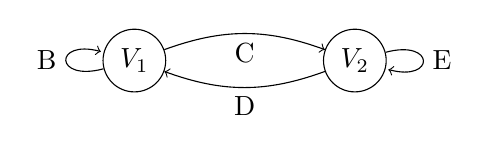
\begin{tikzpicture}[auto, node distance=2.8cm]
        \node[circle, draw=black, name=a]{$V_1$};
        \node[circle, draw=black, name=b, right of=a]{$V_2$};

        \path[->]
            (a) edge [loop left] node {B} (a)
            (b) edge [loop right] node {E} (b)
            (a) edge [bend left=20] node [swap] {C} (b)
            (b) edge [bend left=20] node {D} (a);
    \end{tikzpicture}
    \caption{Rekursions Schema}
    \label{ha2:ueb2:reksceme}
\end{table}

Nun entsprechen die Teilmatrizen in etwa genau dem Kleene Algorithmus. Als neue Matrix $B$ haben wir die Möglichkeit mit $B$ iin $V_1$ zu bleiben,
oder wir gehen mit $C$ in $V_2$ loopen dort mit $E$ und kehren dann mit $D$ nach $V_1$ zurück. Ähnlich gehen wir im neuen $C$ vor. Dort können wir von
und nach $V_1$ loopen und gehen dann einen Schritt nach $V_2$ und können auch dort loopen. Für den unteren Teil analog. Unserer Anschauung und dem Beweis
des Kleene Algorithmuses entsprechend sollten wir so alle möglichen Wege erhalten.
\subsubsection*{(c)}
Wie lässt sich, unter der Berücksichtigung von (a), $A^*$ mit Floyd-Warshall oder mit widerholter Breitensuche brechnen?
Vergleichen Sie die Laufzeiten mit der Laufzeit die Sie in Teil (b) ermittelt haben.\\

\textbf{Lösung:}\\
(1) Da der Floyd-Warshall-Algorithmus eine Matrix der kürzesten Wege (minimale Kosten) ausgibt, gibt es
genau dann einen Weg wenn ein Matrixeintrag kleiner $\infty$ ist.
Sei diese Matrix $\tilde{A}^* = (\tilde{a}^*_{ij})$ eben diese Matrix. Dann erhält man die Matrix $A^* = (a^*_{ij})$ durch
\begin{equation*}
a^*_{ij} = \begin{cases}
              1 & \text{, falls $\tilde{a}^*_{ij} < \infty$} \\
              0 & \text{sonst}
            \end{cases}
\end{equation*}
Der Floyd-Warshall-Algorithmus hat eine Laufzeit von $O(n^3)$ und ist damit schlechter als die Matrizenmultiplikation, die mit $O(n^{2.3blabla}$ Operationen auskommt.\\
(2) Wiederholte Breitensuche:  Man interpretiert die Eingabematrix als Adjazenzmatrix eines Graphen. Eine Breitensuche wird von jedem Knoten aus gestartet um alle
Zusammenhangskomponenten zu finden. Damit kommt man auf eine Laufzeit von $n \cdot (|V| +|E|)$.
Für Graphen mit wenigen Kanten ist diese Laufzeit nahe an $n^2$ (also besser), für Graphen mit vielen Kanten nah an $n^3$ (also schlechter).
\subsubsection*{(d)}

Geben Sie einen efizienten Algorithmus zur Multiplikation von Matrizen an, die nur wenige Einträge $\not= 0$ haben. Analysieren Sie die Anzahl der Operationen
als Funktion der Dimenision $n$ der Matrix und der Anzahl $m$ der Nichtnullelemente.\\

\textbf{Lösung:}\\
Der folgende Algorithmus bekommt als Eingabe zwei $n \times n$-Matrizen $A = (a_{ij}), B = (b_{ij})$.
\begin{lstlisting}[numbers=left]
for i = 1 to n do
  for j = 1 to n do
    tempsum := 0;
    for k = 1 to n do
      if $a_{ik} \neq 0 \land b_{kj} \neq 0$ then
        tempsum := tempsum + $a_{ik} \cdot b_{kj}$
      end
    end
    $c_{ij}$ := tempsum
  end
end
\end{lstlisting}

Wir sehen, dass wir nun nur noch für jedes nicht Nullelement multiplizieren und addieren müssen. Wenn wir es nach oben abschätzen,
müssen wir für jedes nicht Nullelement nur $n$ Multiplikationen und Addition ausführen. Da wir nur arithmetische Operationen zählen
und die Vergleiche nichts kosten erhalten wir so einen Algorithmus mit der Laufzeit $O(m*n)$.\\

Dies erhält die ursorüngliche Laufzeit, da wir bei einer vollbesetzen Matrix $O(n^3)$ Operationen brauchen.
\label{LastPage}
\end{document}
